\section{Review of the calibration problem and calibration methods}
In this section we will summarize \cite{guo2017calibration}'s findings and propositions on the topic of neural network calibration.

\subsection{The general problem of neural network model calibration degradation}
\cite{guo2017calibration} discovered that they could not confirm \cite{niculescu2005predicting}'s observation that neural networks (for binary classification) were typically well-calibrated for the latest generation of deep neural network models. \cite{lecun1998gradient}'s 5-layer LeNet was compared to \cite{he2016deep}'s 110 layer ResNet on the CIFAR-100 dataset. This comparison is visualized in figure \ref{fig:lenet_vs_resnet_calibration_guo_et_al}, where the top row shows prediction confidence histograms and the bottom row shows reliability diagrams (RDs). RDs show a model's accuracy as a function of its confidence. A perfectly callibrated model has a 45° angled line, i.e. the identity function, as its RD. Figure \ref{fig:lenet_vs_resnet_calibration_guo_et_al} shows a striking overconfidence of the ResNet on CIFAR-100 while showing the LeNet has an almost perfect RD on it. \cite{guo2017calibration} thus proposes that the modern ResNet has gained in accuracy over the older LeNet by, through some mechanism, sacrificing calibration. Through abductive reasoning \cite{guo2017calibration} hypothesizes and substantiates that this is a general and explainable evolutionary trend in artificial neural network R\&D that one could call calibration degradation. 

\begin{figure}[htbp!]
  \centering
  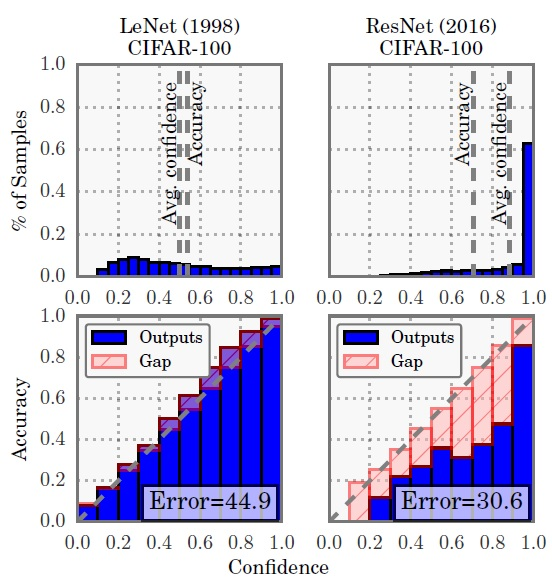
\includegraphics[width=0.6\linewidth]{images/lenet_vs_resnet_calibration_guo_et_al.jpg}
  \caption[5-layer LeNet's vs. 110-layer ResNet's calibration.]{5-layer LeNet (left) vs. 110-layer ResNet (right) calibration.}
  \label{fig:lenet_vs_resnet_calibration_guo_et_al}
  \source{\cite{guo2017calibration}}
\end{figure}
\newpage

\subsection{Formal calibration definitions and metrics}
\cite{guo2017calibration} provide a rigorous definition of and enumerate several metrics for the calibration of supervised multiclass classification.

\subsubsection{Notation and the formal perfect calibration definition}
The input $X \in \mathcal{X}$ and label $Y \in \mathcal{Y}=\{1, \ldots, K\}$ are random variables that follow a ground truth joint distribution $\pi(X, Y)=$ $\pi(Y \mid X) \pi(X)$. Let $h$ be a neural network with $h(X)=$ $(\hat{Y}, \hat{P})$, where $\hat{Y}$ is a class prediction and $\hat{P}$ is its confidence or self-estimated probability of correctness. Neural network $h$ is theoretically defined as perfectly calibrated if and only if equation \ref{eqn:perfect_calibration_in_theory} holds over the ground truth joint distribution $\pi(X, Y)$.
\begin{equation}
  \label{eqn:perfect_calibration_in_theory}
  \mathbb{P}(\hat{Y}=Y \mid \hat{P}=p)=p, \quad \forall p \in[0,1]
\end{equation}

Equation \ref{eqn:perfect_calibration_in_theory} is not practically applicable: $p$ is a continuous variable, therefore equation \ref{eqn:perfect_calibration_in_theory}'s satisfaction cannot be checked in finite time. Equation \ref{eqn:perfect_calibration_in_practice} can instead be used in practice. It is a binning method where predictions are grouped into $M$ equally sized bins over the interval $\interval{0}{1}$ based on their associated confidence.

\begin{align}
  \label{eqn:perfect_calibration_in_practice}
  \operatorname{acc}\left(B_{m}\right) &= \operatorname{conf}\left(B_{m}\right), \quad \forall m \in[0,M] \\ \nonumber
  \text{where}~\operatorname{acc}\left(B_{m}\right) &= \frac{1}{\left|B_{m}\right|} \sum_{i \in B_{m}} \mathbf{1}\left(\hat{y}_{i}=y_{i}\right), \\ \nonumber
  \operatorname{conf}\left(B_{m}\right) &= \frac{1}{\left|B_{m}\right|} \sum_{i \in B_{m}} \hat{p}_{i}, \\ \nonumber
  B_{m} &= \parbox[t]{8cm}{\raggedright The set of indices of samples whose prediction confidence falls into the interval $I_{m}$,} \\ \nonumber
  I_{m} &= \left[\frac{m-1}{M}, \frac{m}{M}\right], \\ \nonumber
  \hat{y}_{i} &= \text{Predicted class label of sample $i$}, \\ \nonumber
  y_{i} &= \text{True class label of sample $i$}, \\ \nonumber
  \hat{p}_{i} &= \text{Confidence of the class prediction of sample $i$}
\end{align}

$\operatorname{acc}\left(B_{m}\right)$ is an unbiased and consistent estimator of $\mathbb{P}\left(\hat{Y}=Y \mid \hat{P} \in I_{m}\right)$ by basic probability theory.

\subsubsection{Calibration metrics}
To make the criterion of perfect calibration, which is a goal that can rarely be reached in practice, useful we need to combine it with a quantitative measure of how close a model is to meeting it. Such a measure then allows us to bring a model ever closer to being perfectly calibrated instead of only to determine whether or not it is so. Three main metrics are layed out by \cite{guo2017calibration} and discussed here. We will call these metrics miscalibration metrics.

\paragraph{Expected Calibration Error (ECE)}
The expected calibration error (ECE), defined by equation \ref{eqn:ece_theoretical}, quantifies miscalibration as the expected absolute difference between the true accuracy of the model given its probabilistic confidence and its probabilistic confidence.
\begin{equation}
  \label{eqn:ece_theoretical}
  \mathrm{ECE}=\underset{\hat{P}}{\mathbb{E}}[|\mathbb{P}(\hat{Y}=Y \mid \hat{P}=p)-p|]
\end{equation}
Equation \ref{eqn:ece_theoretical} cannot be evaluated in practice because $\hat{P}$ is a continuous variable. Therefore equation \ref{eqn:ece_practical}, an approximation-by-binning method similar to equation \ref{eqn:perfect_calibration_in_practice} is used in practice.
\begin{equation}
  \label{eqn:ece_practical}
  \mathrm{ECE}=\sum_{m=1}^{M} \frac{\left|B_{m}\right|}{n}\left|\operatorname{acc}\left(B_{m}\right)-\operatorname{conf}\left(B_{m}\right)\right| \text {, }
\end{equation}
The expected calibration error metric is appropriate for use in model calibration optimization if calibration outliers are acceptable. ECE is ideally 0.

\paragraph{Maximum Calibration Error (MCE)}
The maximum calibration error (MCE), defined by equation \ref{eqn:mce_theoretical}, quantifies miscalibration as the maximum absolute difference between the true accuracy of the model given its probabilistic confidence and its probabilistic confidence.
\begin{equation}
  \label{eqn:mce_theoretical}
  \mathrm{MCE}=\max _{p \in[0,1]}|\mathbb{P}(\hat{Y}=Y \mid \hat{P}=p)-p| \text {. }
\end{equation}
Equation \ref{eqn:mce_theoretical} cannot be evaluated in practice because $\hat{P}$ is a continuous variable. Therefore equation \ref{eqn:mce_practical}, an approximation-by-binning method similar to equation \ref{eqn:perfect_calibration_in_practice} is used in practice.
\begin{equation}
  \label{eqn:mce_practical}
  \mathrm{MCE}=\max _{m \in\{1, \ldots, M\}}\left|\operatorname{acc}\left(B_{m}\right)-\operatorname{conf}\left(B_{m}\right)\right|
\end{equation}
The maximum calibration error metric is appropriate for use in model calibration optimization if calibration outliers are problematic. MCE is ideally 0.

\paragraph{Negative log-likelihood (NLL)}
Negative log-likelihood (also commonly known as cross-entropy loss in deep learning) $\mathcal{L}$ is a standard measure of probabilistic model fit. Equation \ref{eqn:nll_theoretical} gives its definition.

\begin{align}
  \label{eqn:nll_theoretical}
  \mathcal{L} &= -\sum_{i=1}^{n} \log \left(\hat{\pi}\left(y_{i} \mid \mathbf{x}_{i}\right)\right) \\ \nonumber
  \text{where}~\hat{\pi}(Y \mid X) &= \text{The probabilistic model under evaluation,} \\ \nonumber
  n &= \text{The number of samples}
\end{align}
Minimizing equation \ref{eqn:nll_theoretical} brings $\hat{\pi}(Y \mid X)$ ever closer to the true probability distribution. If negative log-likelihood is 0, $\hat{\pi}(Y \mid X)$ is the ground truth probability distribution. We do not use negative log-likelihood in practice to calibrate deep learning models because in this context \cite{guo2017calibration} show that it is too susceptible to overfitting.

\subsection{Calibration methods}
\cite{guo2017calibration} provide and compare several calibration methods we will discuss here.

\subsubsection{Histogram binning}
Histogram binning is a non-parametric calibration method where all uncalibrated prediction confidences $\hat{p}_{i}$ of the dataset are divided into bins $B_{1}, \ldots, B_{M}$. Each bin is assigned a calibrated prediction confidence $\theta_{m}$ such that if $\hat{p}_{i}$ is assigned to bin $B_{m}$, then $\hat{q}_{i}=\theta_{m}$ where $\hat{q}_{i}$ stands for sample $i$'s calibrated prediction confidence. The $\theta_{m}$'s are chosen to minimize the bin-wise squared loss as defined by equation \ref{eqn:histogram_binning} in the case of binary classification.
\begin{align}
  \label{eqn:histogram_binning}
  \min_{\theta_{1}, \ldots, \theta_{M}} &\sum_{m=1}^{M} \sum_{i=1}^{n} \mathbf{1}\left(a_{m} \leq \hat{p}_{i}<a_{m+1}\right)\left(\theta_{m}-y_{i}\right)^{2} \\ \nonumber
  \text{where}~\hat{p}_{i} &= \text{The uncalibrated probability of sample $i$ being positive (1)}
  M &= \text{The number of bins}, \\ \nonumber
  n &= \text{The number of samples}, \\ \nonumber
  1 &= \text{The indicator function}, \\ \nonumber
  0=a_{1} \leq a_{2} \leq \ldots \leq a_{M+1}=1 &= \parbox[t]{5cm}{The boundaries of bin $B_{m}$ defined by the interval $\left(a_{m}, a_{m+1}\right]$,} \\ \nonumber
  \theta_{m} &= \parbox[t]{5cm}{The calibrated prediction confidence associated with bin $m$,} \\ \nonumber
  y_{i} &= \parbox[t]{5cm}{Sample $i$'s true class, either positive (1) or negative (0)}
\end{align}
Typically the bins are either made equally long or sized to equalize the number of samples they contain.
Given fixed bin boundaries, the solution to equation \ref{eqn:histogram_binning} is to let $\theta_{m}$ be equal to the average number of positive-class samples in bin $B_{m}$.

\subsubsection{Isotonic regression}
Isotonic regression is a generalization of histogram binning where not only the calibrated prediction confidences of each bin but also the bin boundaries are optimized, as defined by equation \ref{eqn:isotonic_regression} in the case of binary classification.
\begin{align}
  \label{eqn:isotonic_regression}
  \min _{
    \begin{array}{c}
      M \\
	  \genfrac{}{}{0pt}{}{\theta_{1}, \ldots, \theta_{M}}{a_{1}, \ldots, a_{M+1}}
    \end{array}
  } & \sum_{m = 1}^{M} \sum_{i = 1}^{n} 1\left(a_{m} \leq \hat{p}_{i} < a_{m + 1}\right)\left(\theta_{m} - y_{i}\right)^{2} \\ \nonumber
  \text{ subject to } & 0 = a_{1} \leq a_{2} \leq \ldots \leq a_{M + 1}=1, \\
  & \theta_{1} \leq \theta_{2} \leq \ldots \leq \theta_{M}. \\ \nonumber
  \text{where}~\hat{p}_{i} &= \text{The uncalibrated probability of sample $i$ being positive (1)}
  M &= \text{The number of bins}, \\ \nonumber
  n &= \text{The number of samples}, \\ \nonumber
  1 &= \text{The indicator function}, \\ \nonumber
  0=a_{1} \leq a_{2} \leq \ldots \leq a_{M+1}=1 &= \parbox[t]{5cm}{The boundaries of bin $B_{m}$ defined by the interval $\left(a_{m}, a_{m+1}\right]$,} \\ \nonumber
  \theta_{m} &= \parbox[t]{5cm}{The calibrated prediction confidence associated with bin $m$,} \\ \nonumber
  y_{i} &= \parbox[t]{5cm}{Sample $i$'s true class, either positive (1) or negative (0)}
\end{align}

\subsubsection{Bayesian binning into quantiles (BBQ)}
\subsubsection{Platt and temperature scaling}
\subsubsection{Comparison}

\section{Review of applications of interest}
In this work we want to evaluate and analyze the impact of calibration on representative DeepProbLog use-cases where it presents a considerable issue. Unfortunately, these use-cases are not a given. To find and choose some, we first required that:
\begin{itemize}
  \item using PLP with neural predicates to tackle it is appropriate
  \item it is widely studied in neuro-symbolic integration research
  \item there is room to improve it through callibrating (parts of) models
\end{itemize}
If the first and third criterions are not met, there is no reason to use DeepProbLog and/or calibration and the knowledge we'd gain and features we'd create would not necessarily be relevant to our target audience. That's why we disregard most well-known AI toy problems such as playing chess, the N-queens problem and MNIST digit recognition and we start with reservations about using the DeepProbLog demonstration problems showcased by \cite{manhaeve2018deepproblog}. But we do require widely used challenges like the general AI toy problems so that our work's properties and performance can be easily compared to those of other approaches (\cite{russell2002artificial}), hence our second criterion. \par
We then performed a shallow literature scan of neuro-symbolic integration to find recurring themes and toy problems in this field of research. The scientific literature search engines Google Scholar (by Google) and Limo (by KU Leuven) were used to search for papers containing the keywords "neuro", "symbolic" and "integration" simultaneously. 63 random papers were chosen from the results. A breakdown of the problem categories these papers work in is given in table \ref{subject_breakdown}. Papers can work in multiple categories, the count column shows how many work in the category and the \% column shows what percentage of the 63 work in it.
\begin{table}[!htbp]
\centering
\begin{tabular}{ |c|c|c| }
 \hline
 \textbf{Category} & \textbf{Count} & \textbf{\%} \\
 \hline
 Acoustic information processing & 1 & 1.59\% \\
 \hline
 Actuarial science & 2 & 3.17\% \\
 \hline
 Natural sciences modelling & 2 & 3.17\% \\
 \hline
 Control theory & 4 & 6.35\% \\
 \hline
 Fraud detection & 1 & 1.59\% \\
 \hline
 Natural language processing & 7 & 11.11\% \\
 \hline
 Numerical analysis & 1 & 1.59\% \\
 \hline
 Robotics & 2 & 3.17\% \\
 \hline
 Social \& political sciences & 2 & 3.17\% \\
 \hline
 Symbolic knowledge \& structured data processing & 33 & 52.38\%  \\
 \hline
 Visual information processing & 16 & 25.40\%  \\
 \hline
\end{tabular}
\caption{Subfield breakdown of neuro-symbolic integration research}
\label{subject_breakdown}
\end{table}